\chapter{Evaluation}
\label{cap6}


\section{Applicability of the Pluto framework}\label{applicability}


We developed our programming framework thinking about indoor applications utilizing nano-drones.
Actually, since we work at a sufficiently high level of abstraction, because we can use an API which make the drones navigate in the environment, the model can be extended to almost every kind of drone, aerial terrestrial and aquatic.
So, we can say that the Pluto programming framework is "drone independent", and this greatly extends its applicability, including also outdoor, aquatic and terrestrial environments; it is in charge of the programmer to manage the interaction between Pluto and the specific type of drone he wants to use for the particular application he's developing.

Pluto is fully exploited when there is a team of drones to manage (see \ref{fig:WIS} and \ref{fig:DD}), although it perfectly works also in the case of a single drone (see \ref{fig:OF}).

Since we decided to use a Team-level approach (see \ref{teamlevel}), our model can be used for developing applications where the user can give to the system a set of actions to be performed; the dispatching of these actions is managed by the "central brain", which takes care of assigning the drones to the action and to handle all the exceptions (battery low, crashes etc.). So, the drones are only actuators that perform an action, there is no communication between them, their behavior is monitored and decided by the central brain.

Since drones cannot communicate between them, Pluto cannot be used for applications where drones must perform some kind of action requiring explicit communication or data exchange between them; the logic is managed by the central brain, so communication between drones is always mediated by this component; a drone can send data to the central brain, and this could send again that data to another drone.

Hereinafter we analyzed some already existing example applications, showing whether they can be managed/developed with the Pluto programming framework or not.

\subsection{Alfalfa Crop Monitoring and Pollination}\label{alfalfa}

The Alfalfa Crop Monitoring and Pollination\cite{alfalfa} is a typical example of swarm-level approach application.
Alfalfa is an important food crop for cattle and requires an external pollinator (e.g. bees) to produce seeds. In recent years, colony collapse disorder has devastated honeybee populations and jeopardized the cultivation of important crops.
A swarm of drones can pollinate the alfalfa plants and also monitor them for pests and diseases, trough visual spot checks.
So, the whole application provide three periodic actions: searching for pests, searching for diseases, and looking for flowers in bloom.
Each one of these actions is achieved by taking pictures of the plants.
The user may need to define time constraints within the pollination action must be completed.

The following Pluto Editor graph describes the behavior of the Alfalfa Crop Monitoring and Pollination\cite{alfalfa} application:

\begin{figure}[H]
  \centering
  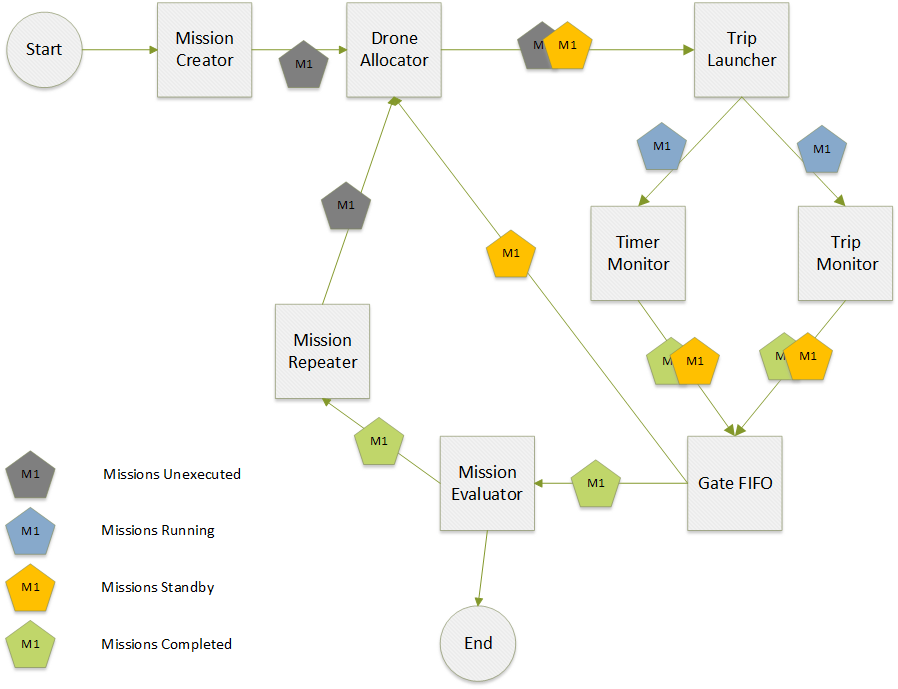
\includegraphics[width=\linewidth]{pictures/Alfalfa_Diagram.png}
  \caption{Pluto graph for the Alfalfa Crop Monitoring and Pollination application}
  \label{fig:alfalfaGraph}
\end{figure}

Thanks to the \textit{Take photo} action, already implemented in Pluto, the drones are able to perform the monitoring of leaves for pests, diseases and flowers in bloom.
\\

As already explained, a Mission object contains a list of trips to be executed.
Since, inside the Mission entity, these trips are performed sequentially, if the user wants to send more than one drone simultaneously on the same location, he has to create more than one Mission.
Indeed missions are executed in parallel, so if the user wants to simultaneously send 3 drones on the same location, he simply has to create three missions.
Then, on the Trips page of each of the three missions, he has to choose the same location.
\\

To concretely choose the specific locations to monitor, the user is provided with a map over which he can drag and drop the action \textit{Take photo}.
\\

The Mission Repeater block takes care of continuously sending the drones to monitor these locations.
Regarding the "Pollination" task, it can be added thanks to the \textit{custom action} feature, through which the programmer can add to the model a brand new Action, making use of a specific external API.
\\

Concerning the pictures evaluation to detect pests, diseases and flowers in bloom, the developer has to add the custom code in the Evaluator class, using again an external API. 
Each photo will have three associated parameters: the boolean attributes \textit{pest}, \textit{disease} and \textit{bloom}.
These attributes are false by default and they are set to true when the leaves are damaged, their color turns greenish-white or the flowers are in bloom, respectively. 
\\

The MissionEvaluator block enables the evaluation of the photos taken by the drones. If the pest and/or disease attributes are true, the system notifies the farmer of the damaged location, adding a log line in the console of the Monitor Page of the Pluto User Interface.
If the bloom attribute is true, a new Trip will be created and the drones will be sent to that location to pollinate the flowers.
\\

The time constraints, which are set by the user thanks to the timer attribute of the Mission entity, will be respected thanks to the TimerMonitor block.
This block takes care of setting the Mission status to FAILED if one of its Trips is not completed within the timer.
\\

The GateFIFO block takes as input two Mission instances, one from the Trip Monitor and the other one from the Timer Monitor.
It takes care of propagating only the first instance that arrives to it.
For example, if the timer has expired then it will propagate the Timer Monitor instance, otherwise the Trip Monitor one.
\\

After the GateFIFO block there is a bifurcation:
if the Mission is completed, it is sent to the MissionEvaluator, otherwise there are some trips of the mission that must be executed again, and so the Mission is sent to the DroneAllocator.
The full explanation of the functionality of each block can be found in section \ref{blocks}.
\\

The following is the code of the Evaluator needed for the development of the Alfalfa\cite{alfalfa} application:
"dataMap" is an hashmap that binds each Trip with the picture. The Trip is the key, which represents the journey performed by the drone and the Photo is the value, which is the picture taken by the drone once the Trip has been completed.
For each photo taken by the drone, if the \textit{pest} or the \textit{disease} attribute are true, the system will signal to the farmer the location where the problem exists, through the log function.
If the \textit{bloom} attribute is true, the plants at that location must be pollinated, so a new Trip is created, its status is set to WAITING, the Action is set to Pollinate and the target location is set to the same location of the Trip where the bloom attribute is true.
Finally the Trip is added to the list of trips of the current mission.
The Mission status is set to STANDBY because there is at least a new inserted Trip to execute.
\\


\begin{lstlisting}
		String result = null;

		// Retrieve all entries of the map, it means we are iterating
        // all the completed Trips that wrote their result in the Evaluator
		for (Map.Entry<Trip, Object> entry : dataMap.entrySet()) {

			// we need to consider only the Trips related to the current
            // mission we are evaluating
			if (missionToEvaluate.getCompletedTrips().contains(entry.getKey())) {
				
				// retrieve the Photo related of the current Trip
				Photo photo = (Photo) entry.getValue();
				
				if (photo.hasPest() || photo.hasDisease())
					
					return "WARNING: Pest/disease at location: "
							+ entry.getKey().getTargetLocation();

				if (photo.hasBloom()) {

					// create a new Trip to pollinate the flowers
					Trip trip = new Trip();
					trip.setName("PollinateTrip");
                    
                    // Set the same target location
                    // of the Trip that has found the flowers
					trip.setTargetLocation(entry.getKey().getTargetLocation());
                    
                    // This action must be implemented by the developer
					trip.setAction(Action.POLLINATE);
                    
                    // the status WAITING means that this Trip
                    // is ready to be launched
					trip.setStatus(Trip.WAITING);

					// adding this Trip to the Trip list
                    // that contains all the Trips to be launched
					missionToEvaluate.getTrips().add(trip);
                    
					// The status STANDBY means that the mission
                    // has some Trips to be launched yet and
					missionToEvaluate.setStatus(Mission.STANDBY);
				}
			}
		}

		// Result is a "success" because all the Photos of this 
        // mission have been evaluated
		result = "Success";
        
		return result;
\end{lstlisting}

The following is a possible source code of the Pollination Action:

\begin{lstlisting}
	// This is the method called by the drone
	// after it reaches the target location
	@Override
	public Object doAction() {
		Pollinator pollinator = System.getPollinator();
		pollinator.pollinate();
		return true;
	}
\end{lstlisting}


To further clarify the development of the Alfalfa\cite{alfalfa} application with Pluto, we now show a real execution of the Alfalfa application in a concrete scenario:
we want to simultaneously send three drones to monitor the plants distributed in a circular area.
So, we create three Mission entities, and, for each of them, we drag and drop the action \textit{Take photo} on the map, in order to create the trips composing the circular area, as shown in figure \ref{fig:alfalfaArea}. Then the drones will take photos over these spots and, in case of bloom, a new Trip will be created to Pollinate the same area.

\begin{figure}[H]
  \centering
  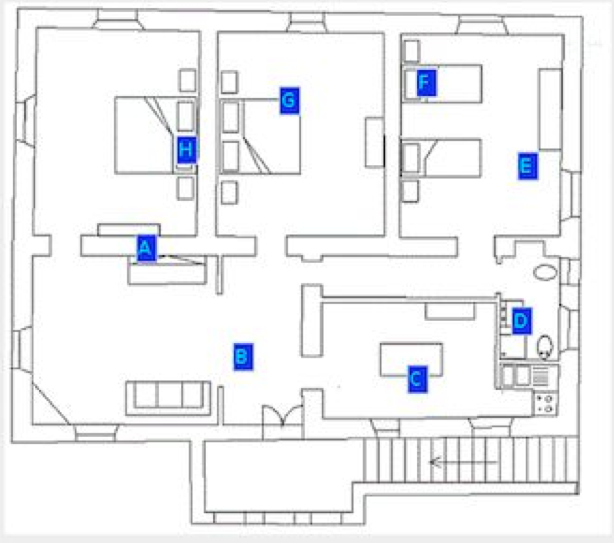
\includegraphics[width=\linewidth]{pictures/alfalfaArea.png}
  \caption{The circular area to monitor}
  \label{fig:alfalfaArea}
\end{figure}


To describe in a detailed way the execution flow, we now show the sequence diagrams of the execution:
\\

 \begin{figure}[H]
   \centering
   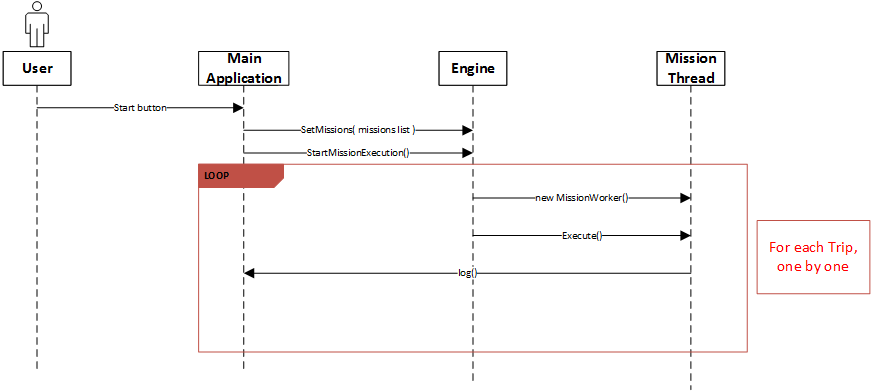
\includegraphics[width=\linewidth]{pictures/Alfalfa_Sequence_MissionStart.png}
   \caption{Sequence diagram of a starting mission}
   \label{fig:alfalfaSequence1}
 \end{figure}

In figure \ref{fig:alfalfaSequence1} are shown the first calls after the user clicks on the Start button in the MonitorPage.
The execution of the Mission starts and a thread is assigned to each Trip of the Mission. The information on the execution of each Trip is sent to the Pluto Main Application and showed to the final user, through the \textit{log()} function.
\\

 \begin{figure}[H]
   \centering
   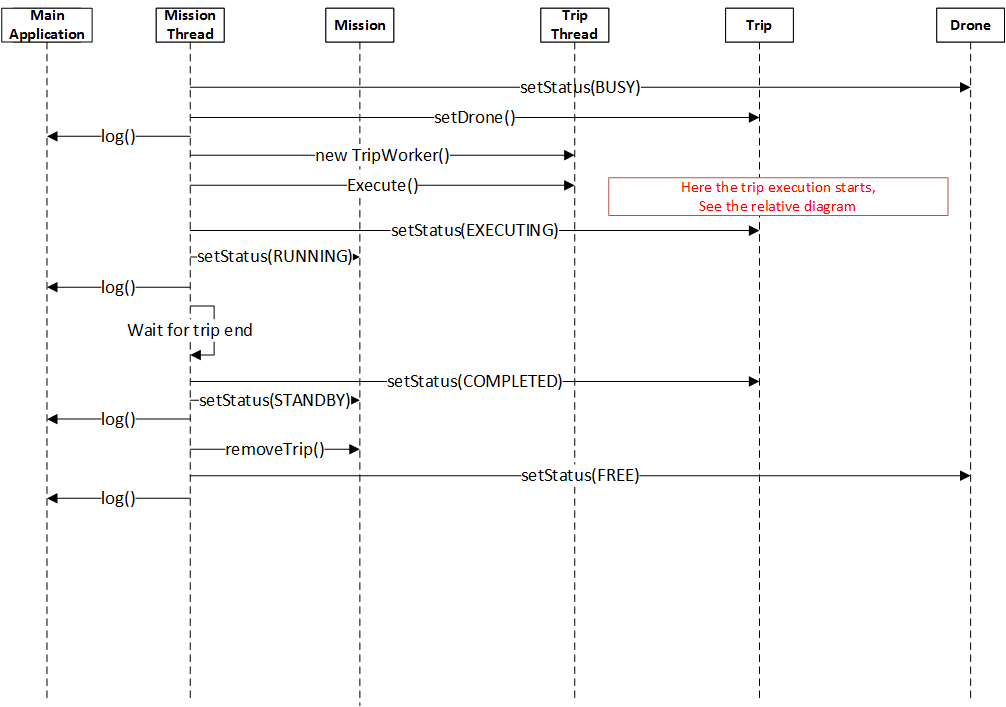
\includegraphics[width=\linewidth]{pictures/Alfalfa_Sequence_MissionExecution.png}
   \caption{Sequence diagram of the mission execution flow}
   \label{fig:alfalfaSequence2}
 \end{figure}

In figure \ref{fig:alfalfaSequence2} is shown the Mission Execution.
The \textit{Mission Thread} component takes care of assigning a drone to the current Trip, setting the status of the drone as BUSY, the status of the Trip to EXECUTING, the status of the Mission to RUNNING.
For each Trip a \textit{TripWorker} instance is created, that simply manage the threads associated to the trips.
Then it waits for the completion of the current Trip, set its status to COMPLETED and the Mission Status to STANDBY, since there are other trips in the list to be executed.
Finally, the completed Trip is removed from the list of trips to be executed and the Drone status is set to FREE
\\

 \begin{figure}[H]
   \centering
   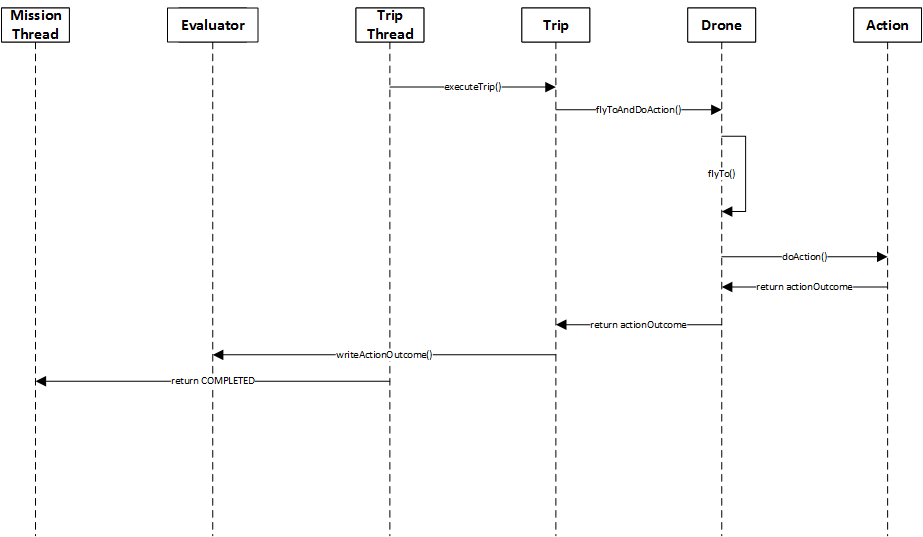
\includegraphics[width=\linewidth]{pictures/Alfalfa_Sequence_TripExecution.png}
   \caption{Sequence diagram of the trip execution flow}
   \label{fig:alfalfaSequence3}
 \end{figure}

In figure \ref{fig:alfalfaSequence3} is shown the Trip execution.
The Drone assigned to the Trip is sent to the established location to take the pictures.
After that, the result is returned to the Evaluator class, where the specific algorithm of the application will perform the evaluation on the pictures captured.
\\

 \begin{figure}[H]
   \centering
   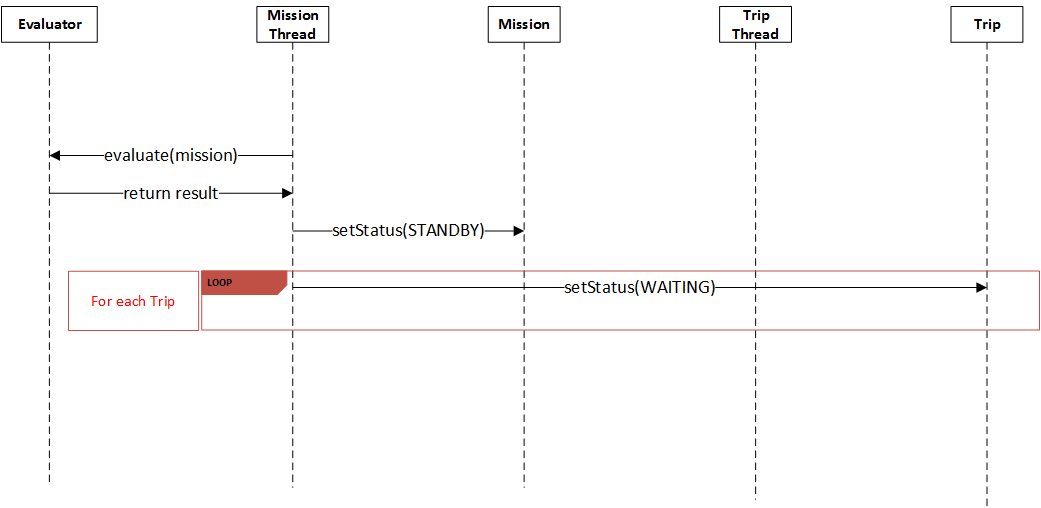
\includegraphics[width=\linewidth]{pictures/Alfalfa_Sequence_MissionEnd.png}
   \caption{Sequence diagram of the mission ending flow}
   \label{fig:alfalfaSequence4}
 \end{figure}

In figure \ref{fig:alfalfaSequence4} are shown the final steps of the Mission execution.
The \textit{Evaluator} will control the pictures taken by the Drone, and it wind that there are some plants to pollinate.
So the Mission status is set to STANBY since new trips will be created to pollinate the plants. The trip status is set to WAITING.
\\

\subsection{Aerial mapping of archaeological sites}\label{aerialMapping}

This application allows archaeologists to survey ancient sites without involving their direct presence on it.
Many Ortophotos of the site are taken, so that the archaeologists can see the geometric layout of the site, without physically walking near it, which could cause irreparable damages.
An orthophoto is an aerial photo that is geometrically-corrected so that distances between pixels are proportional to true distances, such that the photo can be used as a map.
Drones are sent to take a series of ortophotos which then will be stitched together to derive a single ortophoto; if the individual pictures do not have sufficient overlap, the resulting orthophoto will show excessive aberrations, and, in that case, the drone is sent out again to take more pictures.
If the obtained ortophoto is not adequate, the archaeologists should be able to send more drones on that particular area.
The drones must perform their actions in a limited amount of time, since if too much time pass between two ortophotos, the scene may change.

The following figure is the Pluto editor graph needed to create the Aerial Mapping of archaeological sites application. 

\begin{figure}[H]
  \centering
  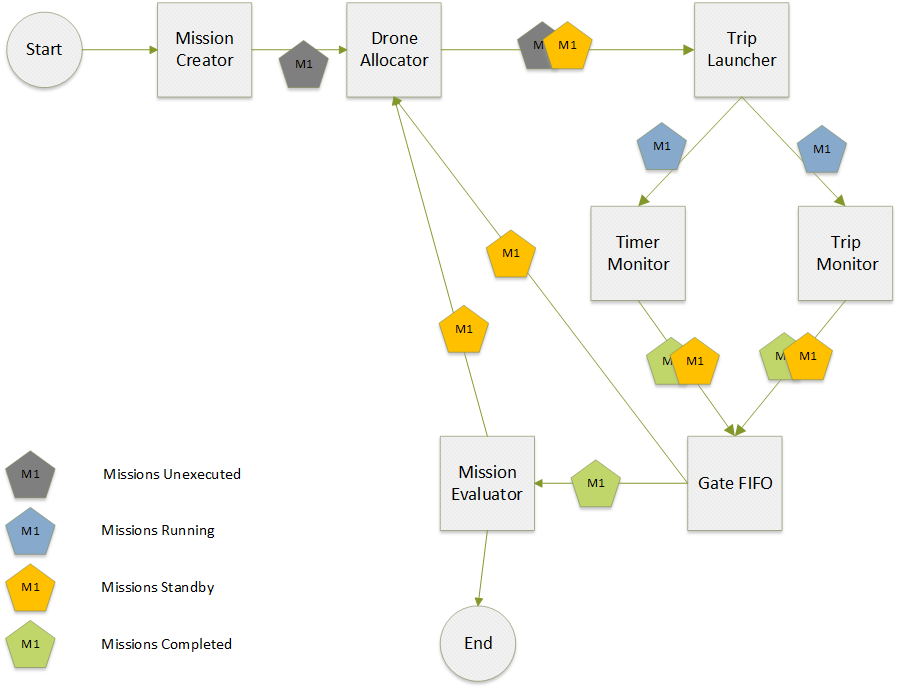
\includegraphics[width=\linewidth]{pictures/Putti_Diagram.png}
  \caption{Pluto graph for the Aerial Mapping of archaeological sites}
  \label{fig:puttiGraph}
\end{figure}

The drones can already take pictures thanks to the \textit{Take Photo} action.
\\

To send the drones to take pictures over the site location, the user has to simply create the Missions entities and add the Trips to the map he will be provided with.
In the case the archaeologists want to send more drones on the locations where they can't obtain an adequate ortophoto, they just have to add more Mission entities.
For example, if one archaeologist want to send 3 drones simultaneously on a particular location, he has to create 3 Mission entities.
Then for each Mission he simply has to drag and drop the \textit{Take photo} action on that particular location.
\\

Thanks to the MissionEvaluator block, that analyzes the drones data at the end of the missions, the Main Application can decide if the photos are good enough or if more drones must be sent out to take new pictures in that specific location.
\\

It is important to underline that, using the Pluto framework, it is not possible to obtain the very same behavior of the original application.
Indeed, two consecutive photos must be taken within a time constraint.
This cannot be fulfilled with Pluto, since the Timer Monitor block deals with a time interval that starts when the drone leaves the base station, ensuring that it will take the picture before the time interval expires.
So, there is no way to state a time constraint between two consecutive photos.
\\

The GateFIFO block takes as input two Mission instances, one from the Trip Monitor block and the other one from the Timer Monitor.
It takes care of propagating only the first instance that arrives to it.
For example, if the timer has expired then it will propagate the Timer Monitor instance, otherwise the Trip Monitor one.
\\

After the GateFIFO block there is a bifurcation:
if the Mission is completed, it is sent to the MissionEvaluator, otherwise there are some trips of the mission that must be executed again, and so the Mission is sent to the DroneAllocator.
The full explanation of the functionality of each block can be found in section \ref{blocks}.



Concerning the code of the Evaluator block needed for the development of the Aerial Mapping\cite{putti} application, as for the previous application, we can find each photo taken during the missions in the "dataMap" parameter, that is an hashmap that create a relation between a Trip and the photo taken through its Action.
First of all, the ortophotos are stitched together to obtain the final ortophoto, trough the \textit{stitch} function.
If the final ortophoto shows excessive aberration, the ortophotos composing it are analyzed and if they don't have sufficient overlap, few new Trips are created with the same target locations of the photos to be taken again. 
The Mission status is set to STANDBY because there is at least a new inserted Trip to execute.
It is important to underline that this application differs from the Alfalfa\cite{alfalfa} one, because the Evaluator algorithm acts in a different way: in Alfalfa\cite{alfalfa} application the algorithm takes care of analyzing the photos of a single mission without considering the others; now, instead, the evaluation needs to merge all the photos of every missions to calculate the aberration. 
The following code snippet shows our implementation of the Evaluator algorithm:
\\
\begin{lstlisting}
		String result = null;
		// The "stitch" method takes a collection of photos as input
        // and return an Ortophoto object derived by a proper algorithm
        // based on the passed photos
		OrtoPhoto ortophoto = stitch(dataMap.values());
		
		if(ortophoto.getAberration() > ABERRATION_THRESHOLD){
			
			// Iteration on the photos that were used in the stitch method
            // to generate the Ortophoto
			for (Photo photo: ortophoto.getPhotoCollection()){
				
				// if the overlap of the single photo is not enough
				if (ortophoto.getOverlapOfGivenPhoto(photo) < OVERLAP_THRESHOLD){
					
					// Loop on all the Trips of every missions
					for (Map.Entry<Trip, Object> entry : dataMap.entrySet()) {
						
						// take the Photo of the current iteration
						Photo p = (Photo) entry.getValue();
						
						// When we found the photo that has the low overlap
						if(photo.equals(p)){
							
							// create a new Trip that will take a new photo
                            // from the same location
							Trip trip = new Trip();
							trip.setName("NewTrip");
							trip.setTargetLocation(entry.getKey().getTargetLocation());
							trip.setAction(Action.TAKE_PHOTO);
							trip.setStatus(Trip.WAITING);

							// add this new trip to the list of trips to be executed
							missionToEvaluate.getTrips().add(trip);
							
							// set the mission status to STANDBY, since a new trip has been created
							missionToEvaluate.setStatus(Mission.STANDBY);
						}
					}		
				}
			}
		}
        
        // All decisions were been chosen so we end the evaluation
		result = "Success";
		return result;
\end{lstlisting}

In order to show the real runtime execution of the Aerial Mapping application with Pluto, we now show a real scenario:
there are 7 drones and 1 big archaeological site to monitor, and we want to send all the drones in that area at the same time to take the ortophotos.
As usual, the user has to create 7 Mission entities.
Then, for each Mission, he has to create the list of Trips by using the map to drag and drop the action \textit{Take photo} on the locations forming the site, shown in figure area3:

 \begin{figure}[H]
 \centering
 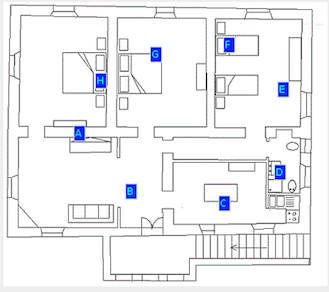
\includegraphics[width=\linewidth, height=8cm]{pictures/area3.png}
 \caption{The archaeological site on the map}
 \label{fig:area3}
 \end{figure}

%sequence


\subsection{PM10}

The PM10\cite{pm10} application is used to build 3D maps of pollution concentration in the atmosphere. 
Initially, there is a predefined 3D grid over which drones are sent to sample the quantity of pollution.
So the drones build a spatial profile of pollution concentration and compute gradients among the areas of higher concentration.
Finally the drones are sent along this gradients to sample the pollution concentration, in order to improve the spatial profile representation.
Any two consecutive samples must be gathered within a given time bound, otherwise the system will take care of speeding up the execution.

The following figure is the Pluto editor graph needed to create the PM10 application:

\begin{figure}[H]
  \centering
  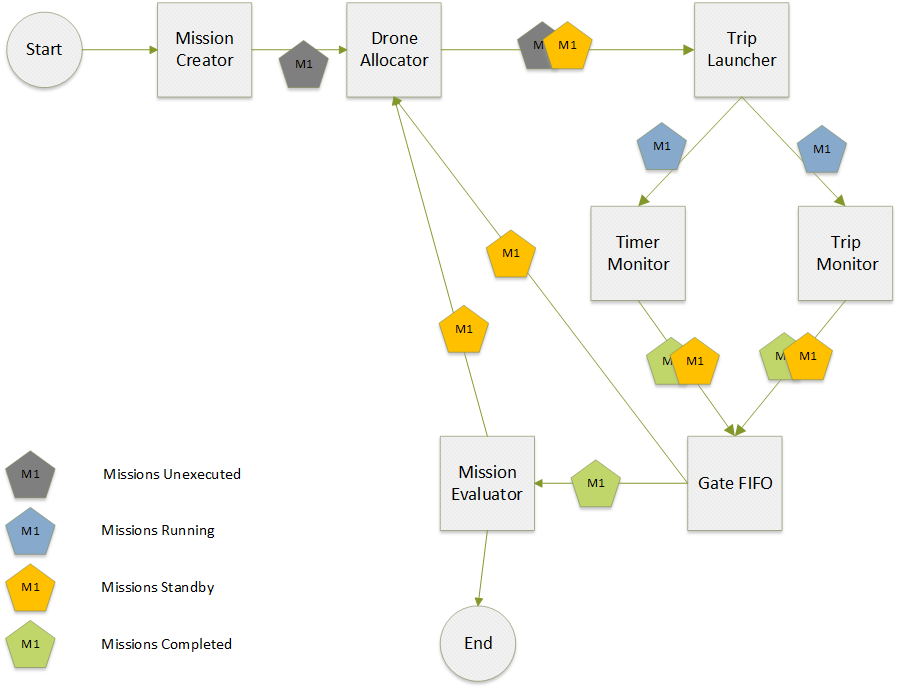
\includegraphics[width=\linewidth]{pictures/Putti_Diagram.png}
  \caption{Pluto graph for the PM10 application}
  \label{fig:pm10Graph}
\end{figure}


For the measurements of pollution quantity, the \textit{measure} action can be used.
\\

The spatial grid must be manually built by the user, organizing the Trips of each Mission on the map he's provided with.
\\

The data collected by the drones are not photos anymore, but a \textit{pollutionQuantity} value which indicates the percentage of pollution in that area.
\\

Then, thanks to the MissionEvaluator blocks, the \textit{pollutionQuantity} variables are confronted and the gradients between areas of higher concentration are computed.
Then the drones will be sent along this gradients, improving the spatial profile.
\\

As for the Aerial Mapping application, shown in section \ref{aerialMapping}, Pluto cannot fulfill the time constraint between two consecutive pollution samples.
As already explained, the timer of Pluto starts when the drone leaves the base station and ensures that it will perform the action within that time interval, but there is no way to constrain the time between two consecutive samples.
\\

The GateFIFO block takes as input two Mission instances, one from the Trip Monitor block and the other one from the Timer Monitor.
It takes care of propagating only the first instance that arrives to it.
For example, if the timer has expired then it will propagate the Timer Monitor instance, otherwise the Trip Monitor one.
\\

After the GateFIFO block there is a bifurcation:
if the Mission is completed, it is sent to the MissionEvaluator, otherwise there are some trips of the mission that must be executed again, and so the Mission is sent to the DroneAllocator.
The full explanation of the functionality of each block can be found in section \ref{blocks}.


Below there is our implementation of a possible Evaluator algorithm:
\\

\begin{lstlisting}
		String result = null;

		// building a new map with only the trip-measure couples of the mission
		// to evaluate
		Map<Trip, Integer> missionMap = new Map<Trip, Integer>();
		for (Map.Entry<Trip, Object> entry : dataMap.entrySet()) {
			if (missionToEvaluate.getCompletedTrips().contains(entry.getKey())) {
				missionMap.put(entry.getKey(), (Integer) entry.getValue());
			}
		}

		// this method use the Trip location and the pollution measure to
		// calculate
		// the gradients and then return a list of String that indicates
		// the positions of these gradients
		List<String> gradientsPositions = calculateGradients(missionMap);

		for (String position : gradientsPositions) {

			// create a new Trip to calculate pollution at the gradient position
			Trip trip = new Trip();
			trip.setName("GradientTrip");
			trip.setTargetLocation(position);
			trip.setAction(Action.MEASURE);
			trip.setStatus(Trip.WAITING);

			// add this new trip to the list of trips to be executed
			missionToEvaluate.getTrips().add(trip);
			// set the mission status to STANDBY, since there are new trips to perform
			missionToEvaluate.setStatus(Mission.STANDBY);
			
		}
			
		// set the result of the evaluation
		result = "Success";
		return result;
\end{lstlisting}


Now we show the execution of the PM10 application with Pluto in a particular scenario:
we have five drones and we want to measure the pollution quantity in the area shown in figure area4 using all of them.
As usual, the user has to create five Missions and to choose the locations of the area to sample through the map of the Trips Page of the Pluto User Interface.
In this way, five drones will monitor simultaneously the area to sample.


%sequence


\subsection{PURSUE}


The PURSUE application\cite{pursue} is representative of surveillance applications. A team of drones monitor an area and they have to follow moving objects which pass through, taking a picture of each one of them when they enter in the camera field.
To do so, drones can operate in two distinct modes: when in "patrolling mode" they simply inspect an area, while when an object is found they switch to "pursuing mode" and start to follow the object.
Since an object could move faster than the drones, no drone can follow it constantly, the system must take care of switching between the real drones in order to constantly follow the target.
There are time constraints to respect between the detection of a moving object and when its picture is taken and, in case of violations,every tracked object with at least one acquired picture is released from tracking, to regain the drone resources and lower the acquisition latency for the next object.
\\

The PURSUE application represents a limit for the Pluto programming framework.
Indeed, in our model, the drones perform their action only at the end of the Trip, so it's not possible for them to actively take a picture in the very same moment the moving object enters in the camera field.
This problem can be lowered by inserting a lot of trips in the area to monitor, with strict time constraints on them, in order to obtain a lot of pictures of the monitored area.
But in this way, not only it's not sure to capture the moving object, but there will be a lot of useless empty pictures.
And, above all, there is still no way for the drones to actively follow the moving objects.

We can conclude that the PURSUE application is too "dynamic" for the Pluto programming framework, and this can be an hint for a future expansion of our work.


\newpage

All the previous applications were already developed and tested with other systems, like Karma\cite{karma} and Voltron\cite{voltron}, but we also developed new applications and tested our framework on them.
We developed the Object-finder (OF), the Warehouse item-finder (WIF)and the Drugs distribution(DD) applications.
In the following subsections we will describe these applications in details, also using a visual representation of their behaviour, and sequence diagrams, to make understand better the whole functioning of each one of them.

\subsection{Object-finder (OF)}

This application will help users to find various objects, in a domestic fashion, like shoes, keys, books etc:

\begin{itemize}
\itemsep2pt
\item{
the user decides which item wants the drones to look for and the area to be inspected
}
\item{
the main system organizes the team of drones, deciding the path for each one of them
}
\item{
the drones fly to the assigned location and, if found, bring the object back to the user, through a magnet or robotic arm
}
\end{itemize}


\begin{figure}[H]
  \centering
  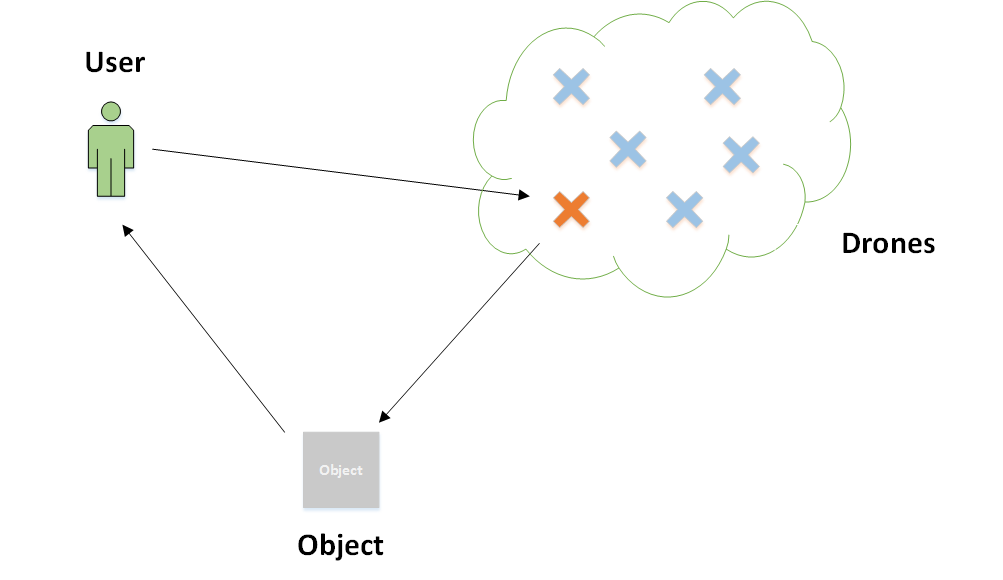
\includegraphics[width=\linewidth]{pictures/OF.png}
  \caption{The basic functioning of the Object-finder application}
  \label{fig:OF}
\end{figure}


\begin{figure}[H]
  \centering
  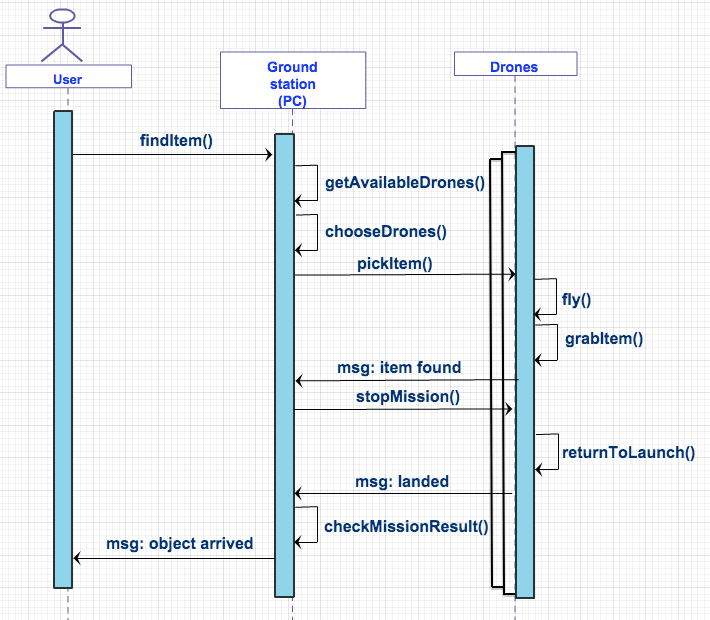
\includegraphics[width=\linewidth, height=8cm]{pictures/OF_sequence.png}
    \caption{Sequence diagram of the Object-finder application}
  \label{fig:OFSequence}
\end{figure}


The user sets which item he needs in the ground station and sends the command; the ground station checks if there are drones unavailable, maybe broken or with low battery status. Then selects the drones that could carry out the mission and send them the command to start the mission. The ground station communicate with each drone, but in the sequence diagram we described the communication only with one of them. After the mission starts, all the drones start looking for the item in the house and when the lucky one finds it, it grabs it and send a notification message to the Ground Station. So, the Ground Station sends a “Stop Mission” message to each drone flying; in this way they could return to the home position. In the end the Ground Station checks if the drone with the item is returned and notifies it to the user.

\newpage

\subsection{Warehouse item-finder (WIF)}

This application will be used to manage a warehouse, taking a list of objects to the user:

\begin{itemize}
\itemsep2pt
\item{
the user makes a list of needed items and writes it on his laptop, tablet or smartphone}
\item{
the main system organizes the swarm of drones and decide which one will take each item in the list
}
\item{
the drones fly to the assigned object and bring them back to the user, through a magnet or robotic arm
}

\end{itemize}


\begin{figure}[H]
  \centering
  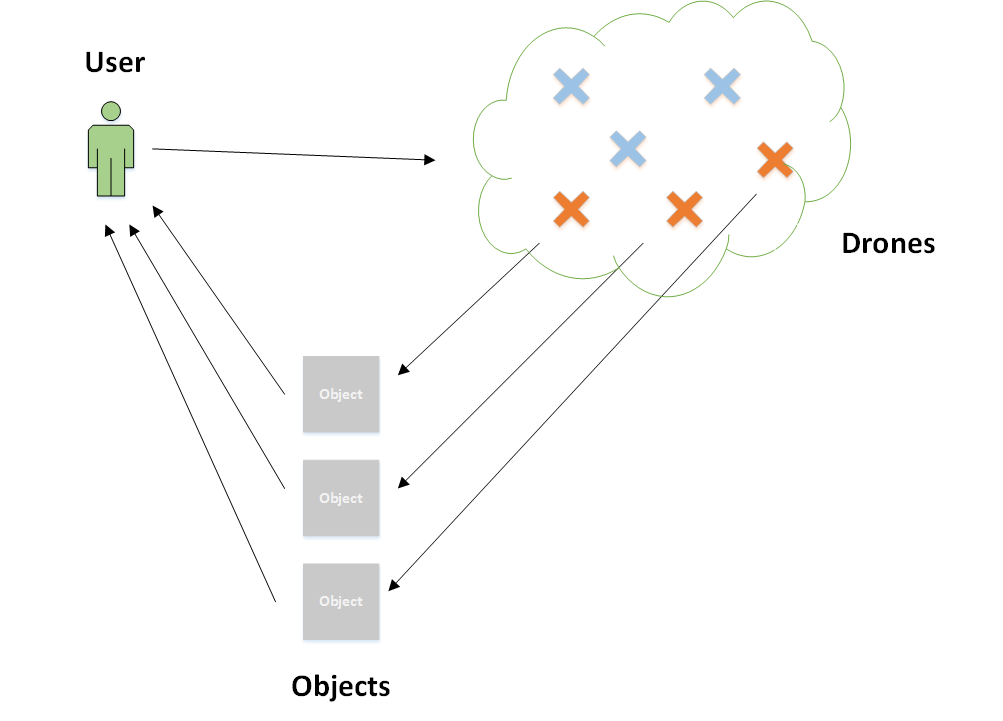
\includegraphics[width=\linewidth]{pictures/WIF.png}
  \caption{The basic functioning of the Warehouse item-finder application}
  \label{fig:WIS}
\end{figure}


\begin{figure}[H]
  \centering
  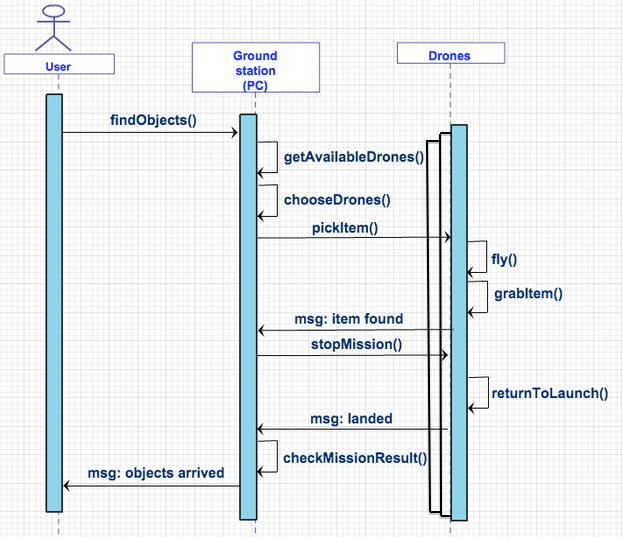
\includegraphics[width=\linewidth, height=8cm]{pictures/WIF_sequence.png}
    \caption{Sequence diagram of the Warehouse item-finder application}
  \label{fig:WISSequence}
\end{figure}

\newpage

\subsection{Drugs distribution (DD)}\label{dd}

This application is thought to assist elders to take their daily drugs, in an hospice context:

\begin{itemize}
\itemsep2pt
\item{
the nurse will prepare a little box with each patient’s daily medicine
}
\item{
each drone, at the right time of the day, will bring the box to his assigned patient
}
\item{
after carrying out their action, the drones return to the start location
}

\end{itemize}


\begin{figure}[H]
  \centering
  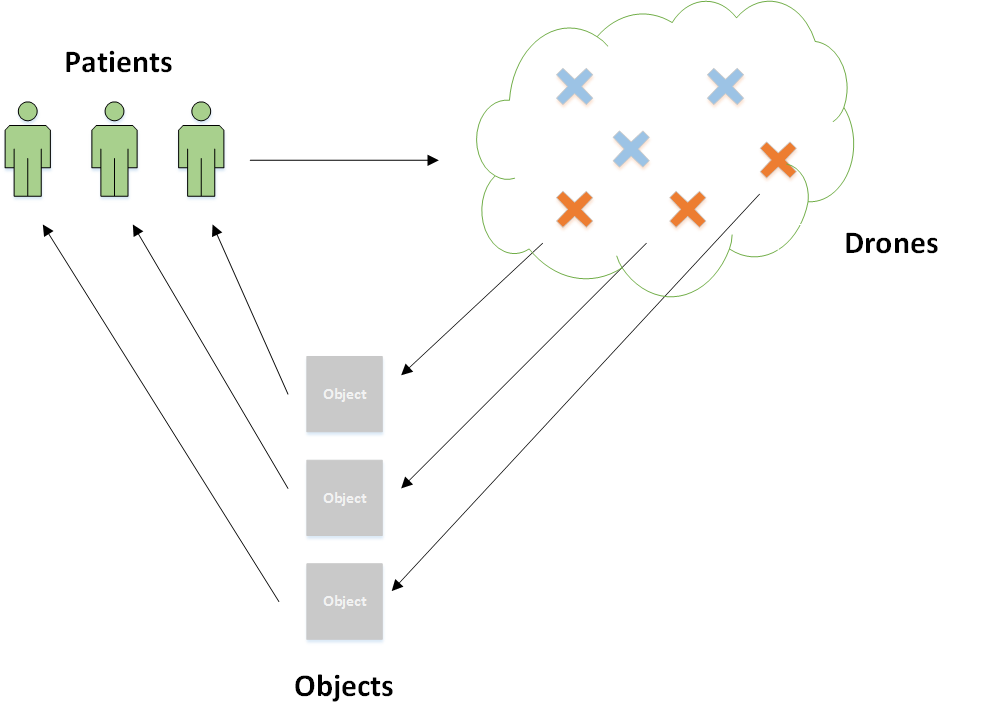
\includegraphics[width=\linewidth]{pictures/DD.png}
  \caption{The basic functioning of the Drugs distribution application}
  \label{fig:DD}
\end{figure}


\begin{figure}[H]
  \centering
  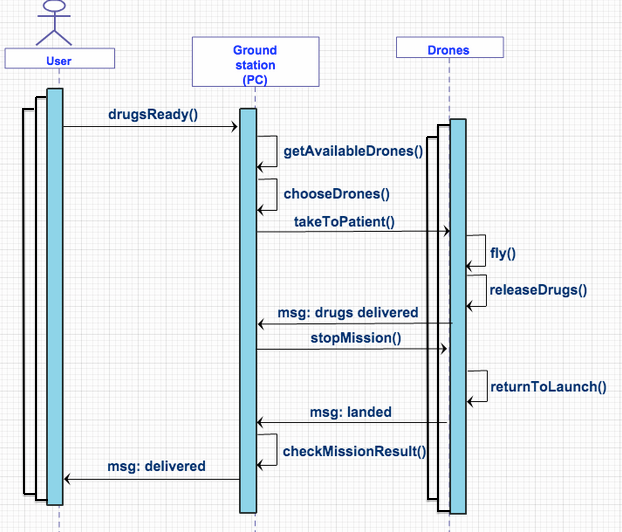
\includegraphics[width=\linewidth,height=8cm]{pictures/DD_sequence.png}
\caption{Sequence diagram of the Warehouse Drugs-distribution application}
  \label{fig:DDSequence}
\end{figure}



The OF,WIF and DD applications can be easily developed with the Pluto editor.
Their basic versions are represented by the basic graph of each application, shown in figure (see \ref{fig:firstStep}),and they can be possibly enriched with the Priority Manager and Timer Monitor blocks, in order to improve the priority of the failed trips or to give a time constraint within the trips must be executed.

\newpage

\section{Usability of the model}
\label{usability}

To evaluate the concrete usability of the Pluto programming framework, we decided to test it on real people, proposing them two "exercises".
The testers were recruited in the "Politecnico di Milano" and "SICS Swedish ICT" environment, in order to guarantee a solid development background and to avoid possible lack of programming knowledge.
We created one exercise for each component of Pluto framework.
The first one consists in the development of an application using the Pluto Graphical Editor.
The exercise is split in three levels, starting from a very basic version and going through more difficult versions. Each version asks the user to add a new functionality by using the available components in the Editor.
The second exercise, instead, asks the user to use the generated code from the previous exercise to run the Pluto Main Application, then asks to create some missions and, in the end, to run them.
The application we choose for the exercises is the Drugs Distribution, already described in section \ref{dd}, because it's very suitable for the type of evaluation we want to perform.
Indeed its basic version can be extended with many features, for example using the Mission Modifier block (section \ref{mm}), and this is exactly our purpose.
The results are shown in section \ref{surveyResult}.
After the execution of the exercises, we asked the users to leave a feedback, proposing them a survey, built according to some metrics that we have defined and that we describe in section \ref{survey}.

\subsection{Proposed exercises}
\label{exercise}

We give the user a complete and sound explanation of the Pluto programming framework, showing how the graphical editor works (shown in section \ref{plutoGraphicalEditor}) and giving him the list of the available entities (shown in section \ref{entities}) and of the implemented blocks (shown in section \ref{blocks}), together with an explanation of the meaning and functionality of each one.
The same explanations are given for all the components of the Pluto User Application (shown in section \ref{plutoMainApp}).

\subsubsection{First Exercise}

The exercise proposes the development of the Drugs Distribution application (shown in section \ref{dd}) in three different versions, increasingly harder to implement:

\begin{itemize}
\itemsep2pt
\item{
\textit{basic version}: we ask the user to implement the basic version of the Drugs Distribution application
}
\item{
\textit{medium version}: we ask the user to raise the priority of the failed trips and to re-insert them in the queue of next trips to be launched, and to add a delay for the trips.
}
\item{
\textit{hard version}: we ask the user to add a time constraint within each trip must be completed, that is the same feature implemented by the Timer Monitor block, but using the Mission Modifier block.
}
\end{itemize}

To solve the first part of the exercise, the user has to create the graph shown in figure \ref{fig:firstStep}, that represents the very basic scheme of each application, since it uses only the basic blocks.
Once created the graph, the user has to right click on the panel and choose "generate code" to accomplish the first step of the exercise.
This is a very easy task to perform, but we think it's useful, because make the user confident with the basic features of Pluto, such as the basic blocks and the code generation mechanism.


\begin{figure}[htb]
  \centering
  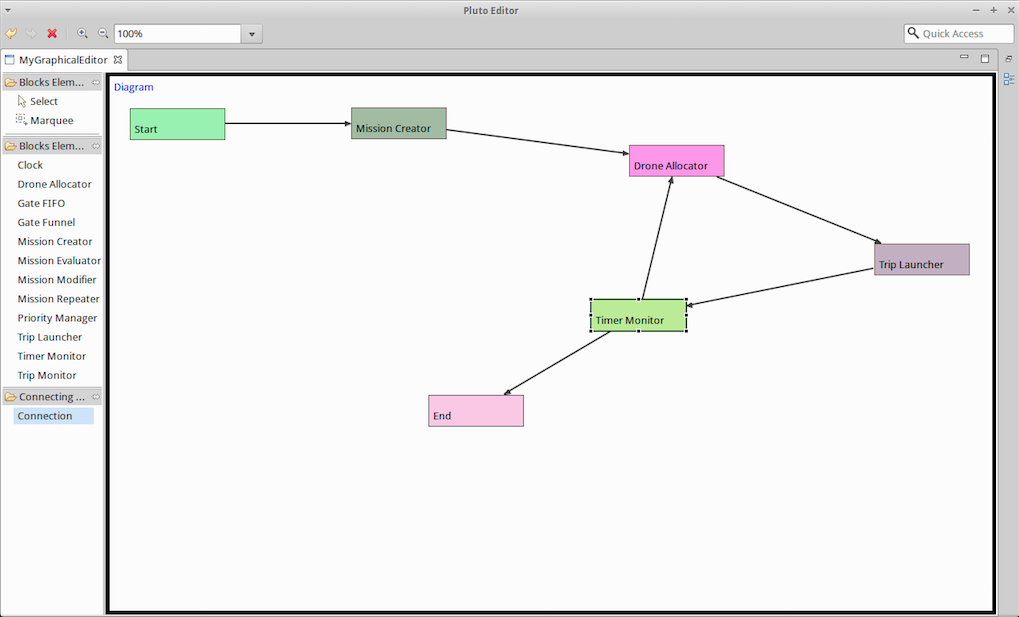
\includegraphics[width=\linewidth]{pictures/EditorScreen.png}
  \caption{Solution of the first step}
  \label{fig:firstStep}
\end{figure}

\newpage

To solve the first part of the second step of the exercise, the user has only to understand that the functionality to add is already implemented by the Priority Manager block, so he has only to add this block to the graph in the right point.
Since we ask him to re-insert the failed trips in the queue of unexecuted trips he has to put the block between the Trip Monitor and the Drone Allocator, as shown in figure \ref{fig:secondStepPriority}.

\begin{figure}[htb]
  \centering
  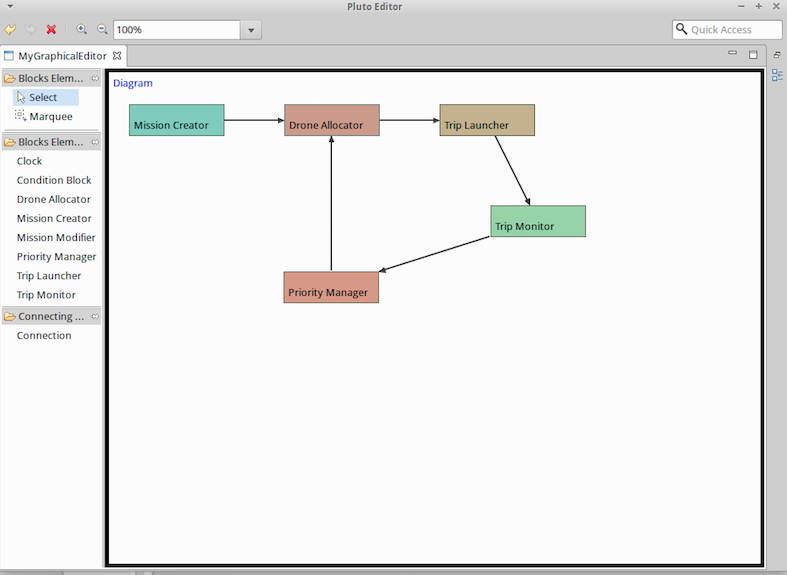
\includegraphics[width=\linewidth,height=7cm]{pictures/secondStep.png}
  \caption{Solution of the second step with Priority Manager}
  \label{fig:secondStepPriority}
\end{figure}

Then to add the Delay feature in the diagram the user needs to do the same thing with the Clock block, that provides the feature to wait for an amount of time, set in the delay attribute of a Trip. This block is taking as input the mission provided by the Trip Monitor and the by the Mission Creator then, after the delay time has passed, gives the mission to the DroneAllocator block, as shown in figure \ref{fig:secondStepClock}.

This is a useful step to compute, because the user learns how to use the connection element, that is a very important feature in the Pluto framework, and also the Priority Manager and Clock blocks.

\begin{figure}[htb]
  \centering
  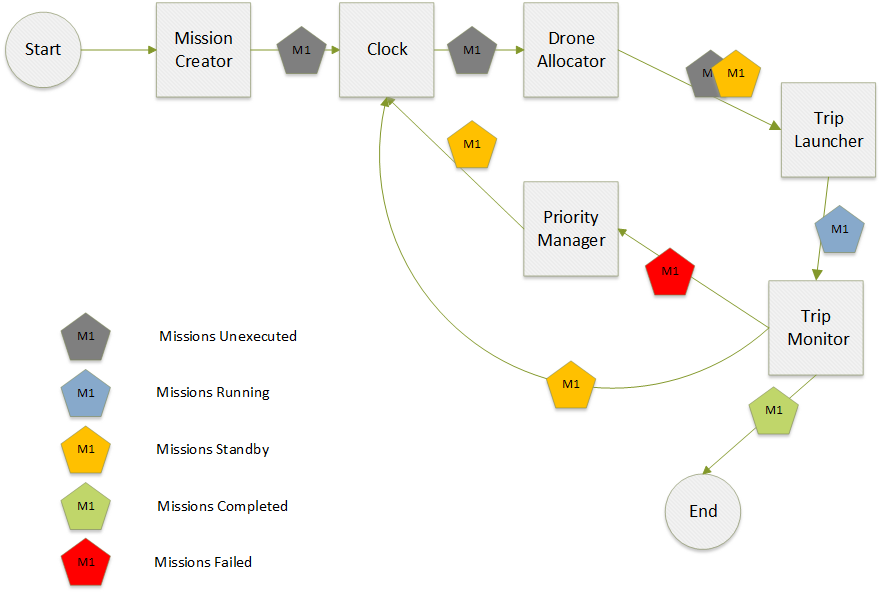
\includegraphics[width=\linewidth,height=7cm]{pictures/secondStepClock.png}
  \caption{Solution of the second step with Clock block}
  \label{fig:secondStepClock}
\end{figure}

\newpage

For the third step, the user has to implement the feature of the Timer Monitor block without using it.
So, he has to use the Mission Modifier block, through which he can insert his code in the application, and put it between the Trip Launcher and GateFIFO blocks, in parallel with the TripMonitor, as shown in figure \ref{fig:thirdStep}.
This is a very useful step to compute, because the user learns how to use Mission Modifier block, which is an important feature of the Pluto Editor, because it allows the programmer to insert his custom code to characterize the application.

\begin{figure}[H]
  \centering
  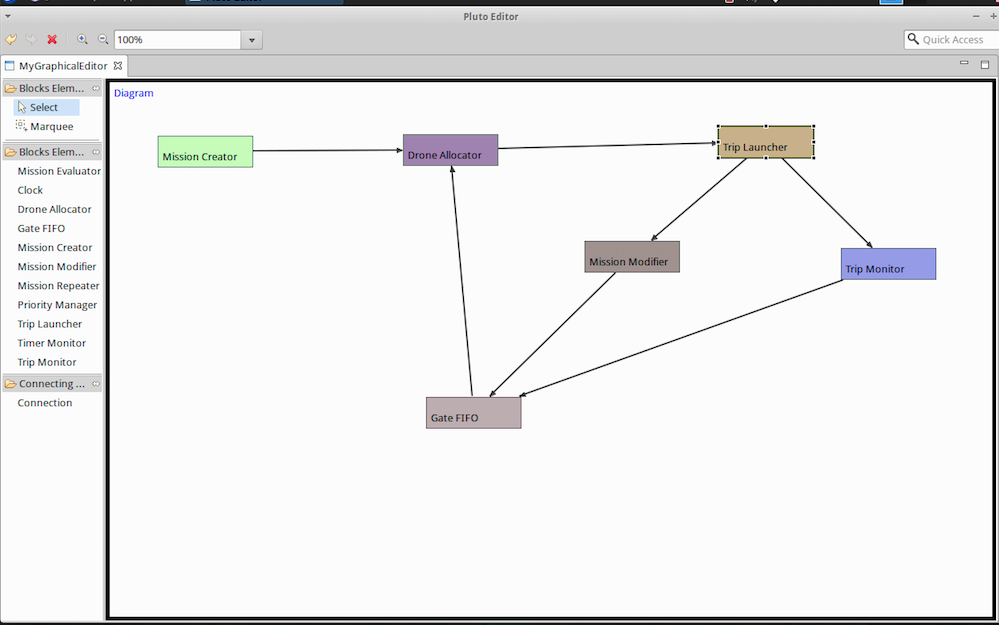
\includegraphics[width=\linewidth, height=8cm]{pictures/thirdStep.png}
  \caption{Solution of the third step}
  \label{fig:thirdStep}
\end{figure}

\subsubsection{Second Exercise}

The main purpose of this exercise is to underline possible issues in the code generated with the Pluto Graphical Editor. We must be sure that all the functionality described by the diagram are enabled in the generated code and that the missions execution will run smooth as the user expects. Any lack in the user experience may compromise the usability of the entire application, so it is important to evaluate the User Interface too. In this way, we check if the visual disposition of the graphics elements is appropriate.
The first step asks every user to create and run the same kind of missions, as described in the following list:

\begin{itemize}
\item Mission 1
	\subitem Trip A -> Action: Take Photo
    \subitem Trip B -> Action: Take Photo
    \subitem Trip C -> Action: Take Photo
\item Mission 2
	\subitem Trip A -> Action: Measure
    \subitem Trip B -> Action: Measure
\item Mission 3
	\subitem Trip A -> Action: Pick Item
    \subitem Trip B -> Action: Release Item
    \subitem Trip C -> Action: Take Photo
    \subitem Trip D -> Action: Measure
\end{itemize}

The location in the map of the Trips was not important while testing, so the tester could decide any place.
In the second step the users were asked to open the Monitor Page and to start the missions following their execution using the provided table and console.
The third step of the exercise consists in calling back the Drone with an RTL command.


\subsection{Evaluation metrics}\label{metrics}

To concretely evaluate the usability of the Pluto programming framework we defined the following metrics, which we applied for both exercises:

\begin{itemize}
\item {Number of people who correctly solved the first part of the exercise}
\item {Number of people who correctly solved the first and second parts of the exercise}
\item {Number of people who correctly solved the whole exercise}
\item {Mean time for the resolution of the first part of the exercise}
\item {Mean time for the resolution of the second part of the exercise}
\item {Mean time for the resolution of the third part of the exercise}
\item {Mean time for the resolution of the whole exercise}
\item {Number of people who solved the whole exercise, but in a wrong way}
\item {Number of people who could not solve the exercise at all}
\end{itemize}

Through metrics 1,2 and 3 we can understand which parts of the exercises are not clear for the user and/or too difficult to implement. 
Through metrics 4,5,6 and 7 we can understand, once the user has understood how to implement each feature, how much is difficult to solve each part of the exercises by measuring the time required to solve each step.
Through metrics 8 and 9, finally, we can understand how easy is to confuse the specifications and how many people couldn't solve any step of the exercises.


\subsection{Baseline}

We want to demonstrate the effective usefulness of the Pluto programming framework, so we decide to compare its features with the API of the Crazyflie Nano-quadcopter, which was described in section \ref{crazyflie}.

Actually, the crazyflie is the drone we chose to use for our applications case study, and we want to demonstrate that, without Pluto and using only the Crazyflie API would be more difficult to build the same kind of applications.

So we decide to propose another exercise to our users, but this time they can use only the Crazyflie API and they have a limited amount of time.

The Crazyflie API is written in Python, so we address to people who knows Python language features.

The exercise consists in make the drone moving from a point A to a point B on a map, performing a single Trip.

It may seem easy, but it can can take a long time to fully understand and apply the API in the correct way.


\subsection{User Survey}\label{survey}

Since we want to evaluate the usability of Pluto, we propose a survey, partly showed in figure \ref{fig:survey}, to the users, in order to understand how easy it is to use and which modifications should be applied to improve the user experience.

\begin{figure}[H]
  \centering
  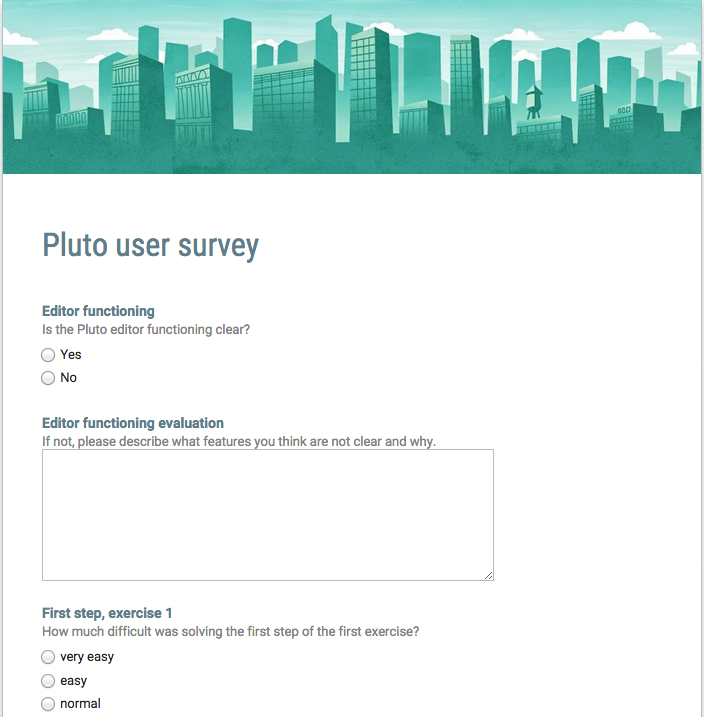
\includegraphics[width=\linewidth]{pictures/survey.png}
  \caption{Pluto user survey}
  \label{fig:survey}
\end{figure}

We ask users to tell us how easy was the development of the various steps of the exercises, and to provide us with a feedback on the usability of the editor and the main application underlining any problems found.
We also ask for suggestions to improve the usability of Pluto.

The survey can be found following this link:

\url{https://docs.google.com/forms/d/1b_52e7VLuns6AH1jiT3TeIRZ_KPRTLJYJe9ckrJanWY/viewform?usp=send_form}


Actually, this survey gives us very useful information about the Pluto framework. We can understand how "usable" it is and which modifications should be performed to improve the user's experience, also thanks to the visualization of the answers in a graphical way, shown in the next section, the \ref{surveyResult}.
Through the questions on the exercises development we can understand how difficult it is to create, modify,customize and execute a particular application, validating "on field" the use of the various blocks, especially the Mission Modifier, and the usability of the user interface.

\subsection{Final Results}\label{surveyResult}

Thanks to the combination of the answers to the user survey of section \ref{survey} and the numeric data collected according to the metrics defined in section \ref{metrics}, in this section we can show the results of the Pluto evaluation.
We make use of graphical representation in order to make the results clearer and easily understandable by everyone.
The metrics data are put into a table, while the results of the user survey are presented with graphics.

%qui vanno i dati delle nostre metriche, in una tabella

%qui vanno i grafici a torta che crea google survey

%qui un nostro commento sui risultati


\newpage

\section{Performance evaluation}\label{performance}

In order to strengthen the evaluation of Pluto, after the user study, described in Section \ref{usability}, we evaluated some qualitative metrics. These metrics are divided in two main types: software metrics and hardware consumption metrics. The former let us know the complexity of our software, on the other hand, the latter are useful to underline possible issues at run-time such as thread deadlock or a too high memory consumption.
Since our framework is composed by two main components, we decided to split this evaluation in two parts: this means that each kind of evaluation was performed on Pluto Graphical Editor first and then on Pluto Main Application.
To measure these parameters we used a very useful tool called VisualVM, shown in figure \ref{fig:visualVM}. 

\begin{figure}[H]
  \centering
  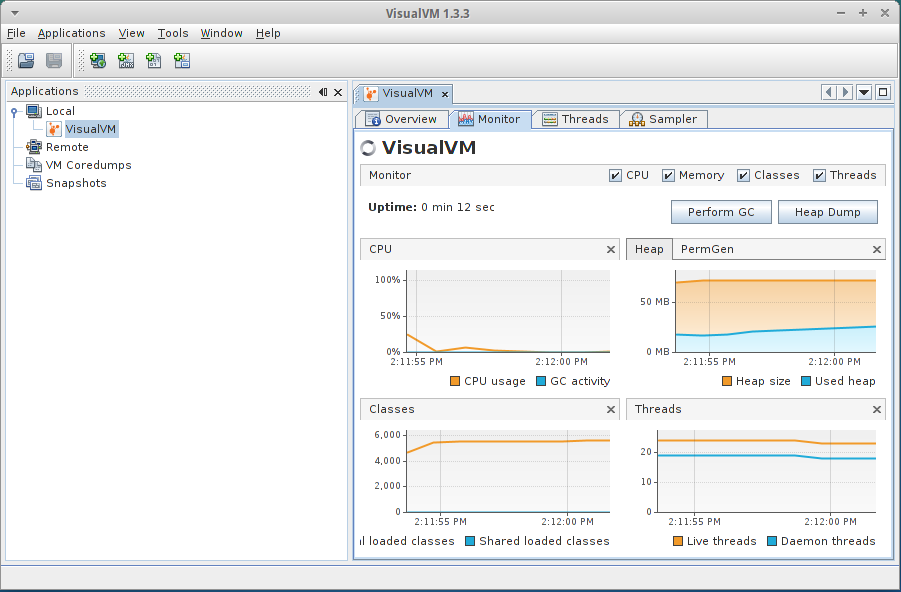
\includegraphics[width=\linewidth]{pictures/visualVM.png}
  \caption{VisualVM interface}
  \label{fig:visualVM}
\end{figure}

It let the user have a global monitoring of the running Java application in your local Java Virtual Machine, at run-time. Furthermore, it has a useful feature that records the profiling of an application in a dump file so that the user can compare different dump files concerning different application sessions.
Then, in the Result section \ref{metricsResult}, we describe the outcome of the tests for Pluto Graphical Editor and Pluto Main Application separately.

\subsection{Software Metrics}

The software metrics let us understand the complexity of the software, we decided to record these parameters for each component of Pluto Framework:

\begin{itemize}
\item Lines Of Code (LOC)
\item Number of classes attributes
\item Number of methods
\item Number of methods calls
\item ...
\end{itemize}

\subsection{Hardware Consumption}

The hardware metrics are those parameters measured at run-time, during the execution of the two software, to check if it generates any performance issues, because it could require too much resources to run smooth. These metrics are:

\begin{itemize}
\item CPU Load
\item Memory Consumption
\item Threads Generated
\item Threads Zombies (not terminated)
\item ...
\end{itemize}

The profiling of the application were done on a machine with these specs:

\begin{itemize}
\item CPU: Intel i7 2640
\item RAM: 4GB
\item VGA: Nvidia GeForce 610M
\item SSD: Kingston 120GB
\item OS: Xubuntu 14.04
\end{itemize}

Concerning the Pluto Graphical Editor, we measured those parameters while creating a lot of blocks and a very complex web of connections, shown in figure \ref{fig:stressDiagram} and then we observed the stress level while generating the source code of the Main Application from that drawing. We concentrated the evaluation on two parameters: the number of blocks and the number of connections. Firstly we fixed the former and we incremented the latter by a step of 5. Then we did the same operation fixing the number of connection and raising the number of blocks.

\begin{figure}[H]
  \centering
  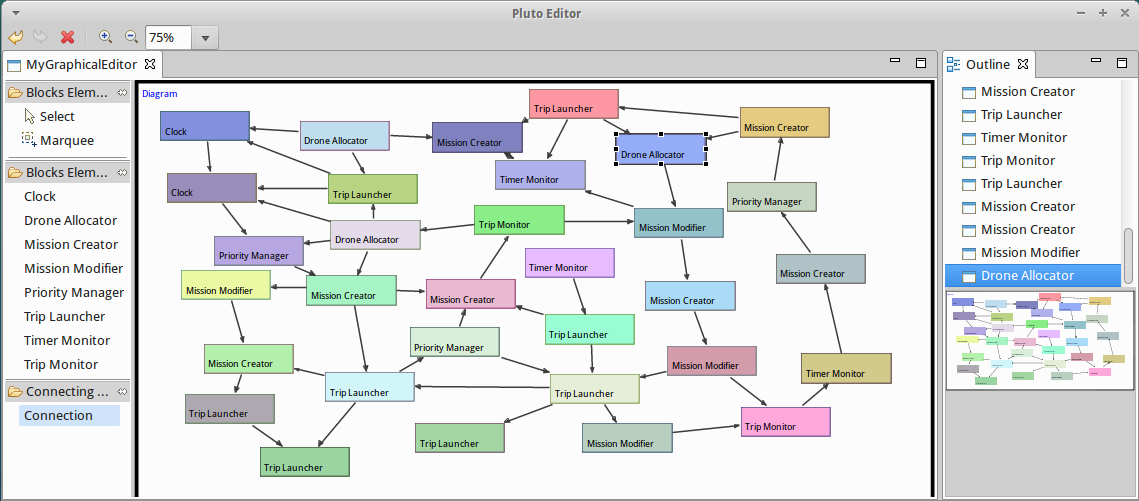
\includegraphics[width=\linewidth]{pictures/stressDiagram.png}
  \caption{Very Complex Diagram Example}
  \label{fig:stressDiagram}
\end{figure}

Furthermore, we evaluated the same metrics concerning the Main Application. We decided to focus this evaluation varying 3 important parameters: the number of Mission, the number of Trips related to a single Mission and the number of available Drones. We started fixing two of these parameters and raised the third step by step. Then we did again this procedure fixing another couple of parameters and varying the left one. In this way, we could evaluate the performance of the Main Application in an accurate way and the result are shown in next section \ref{metricsResult}.

\subsection{Result}
\label{metricsResult}

For software metrics there will be a table with 2 column and each row will be a metric: LOC, classes, ... The 2 columns are Editor and Main app.
\\
For the Performance part of the Editor there will be 2 graph, one with Connecton fixed and number of block raising up, the second is inverted. on X there will be the variable parameter and on Y the metrics: cpu, memory,...
For the performance part of the Main App, there will be 3 graphs: one with Mission and Trip fixed, then Drones will raise by a step of 5 starting from 1. On the X coord there will be Drones, on the Y coord there will be the metrics: cpu consume, memory usage, threads allocated, each line with a different color.
Then the same thing with Mission free, and then with Trip free.



